% =============================================================================
% preprint_recd_ontology_dengue_zenodo_v1.2.tex
% RECD + Ontología del Presente (Tau Sistémico)
% Version 1.2 — June 2026
% Author: Dr. Johel Padilla Villaunueva
% Repository: https://github.com/johelpadilla/ontologia-presente/
% =============================================================================

\documentclass[11pt,a4paper]{article}

\usepackage[margin=1.0in,top=0.85in,bottom=0.85in]{geometry}
\usepackage[T1]{fontenc}
\usepackage{lmodern}
\usepackage{setspace}
\onehalfspacing
\usepackage{microtype}

\usepackage{titlesec}
\titleformat{\section}{\large\bfseries}{\thesection}{1em}{}
\titleformat{\subsection}{\normalsize\bfseries}{\thesubsection}{1em}{}

\usepackage{enumitem}
\setlist[itemize]{leftmargin=*,itemsep=0.25em,topsep=0.2em}
\setlist[enumerate]{leftmargin=*,itemsep=0.25em,topsep=0.2em}

\usepackage{url}
\usepackage{hyperref}
\hypersetup{
    colorlinks=true,
    linkcolor=black,
    urlcolor=blue,
    citecolor=black,
    pdfauthor={Dr. Johel Padilla Villaunueva},
    pdftitle={RECD + Three-Layer Ontology for Early Warning of Dengue Outbreaks (v1.2)},
    pdfsubject={Early-warning systems, complex systems, dengue, recurrence quantification},
    pdfkeywords={early warning systems; complex systems; recurrence quantification analysis; dengue; ontological layers; Joint episodes; synthetic validation}
}

\usepackage{fancyhdr}
\pagestyle{fancy}
\fancyhf{}
\fancyhead[L]{\footnotesize RECD + Ontolog\'ia del Presente (Tau Sist\'emico)}
\fancyhead[R]{\footnotesize Preprint v1.2 -- Zenodo}
\fancyfoot[C]{\footnotesize\thepage}
\renewcommand{\headrulewidth}{0.4pt}

\usepackage{amsmath}
\usepackage{booktabs}
\usepackage{tcolorbox}
\tcbuselibrary{skins,breakable}

\newtcolorbox{zenodolletter}{
    colback=gray!4!white,
    colframe=black!60,
    boxrule=0.5pt,
    arc=2pt,
    left=5pt,
    right=5pt,
    top=3pt,
    bottom=3pt,
    fonttitle=\bfseries\small,
    title=Letter to the Zenodo Reader,
    breakable
}

\title{\textbf{Early warning of dengue outbreaks using Joint episodes from a three-layer ontological framework and calibrated confidence scoring}\\[0.35em]
\large From recurrence to reorganization: A three-layer ontological framework and operational early-warning system for dengue using Joint episodes (C1 + C2) with synthetic validation for data-scarce regimes}

\author{
    \textbf{Dr. Johel Padilla Villaunueva} \\[0.25em]
    \small Ontolog\'ia del Presente (Tau Sist\'emico) Research Program
}

\date{17 June 2026 \\ \small Version 1.2 — Preprint for Zenodo}

\begin{document}

\maketitle

\begin{abstract}
\noindent Effective early-warning systems for dengue are constrained by the absence of mechanistically grounded analytical units that connect local dynamical processes to outbreak-scale reorganization. We introduce a three-layer ontological framework in which Capa 1 denotes local intensification (high recurrence-based M and trapping time), Capa 2 represents sustained permeability (low antisynchrony), and Capa 3 corresponds to detectable structural reorganization. The fundamental unit of analysis is the \textbf{Joint episode}—a coherent interval of Capa 2 containing Capa 1 intensification—which serves as the basis for a single, actionable alert per episode accompanied by an interpretable Confidence Score.

Because only 11 Joint episodes were recovered for San Juan and 3 for Iquitos in the historical record, we developed a controlled synthetic generator to produce realistic Capa 1 + Capa 2 configurations. Three regimes were simulated: San Juan-like (high-intensity, frequent Capa 2), Iquitos-like (low-intensity, rare sustained Capa 2), and noisy balanced. Evaluation of alternative weightings for the Confidence Score demonstrated that duration- and Joint-Score-weighted configurations performed best under high-prevalence conditions (Alto F1 up to 0.55). In the Iquitos-like regime, however, no episodes reached the “Alto” category and mean confidence remained low, indicating that Iquitos represents a qualitatively distinct dynamical regime rather than a simple data-scarcity problem.

The pipeline advances both conceptual coherence and operational utility by replacing per-timestep classification with episode-level alerts and categorical prioritization. All code, synthetic datasets, and protocols are available in the associated repository.

\vspace{0.2em}
\noindent\textbf{Keywords:} early warning systems; complex systems; recurrence quantification analysis; dengue; ontological layers; Joint episodes; synthetic validation; confidence calibration.
\end{abstract}

% =============================================================================
% LETTER TO THE ZENODO READER
% =============================================================================
\begin{zenodolletter}
This preprint presents a mature computational pipeline for early warning of dengue outbreaks, developed within the RECD + Ontología del Presente (Tau Sistémico) research program. The work integrates a three-layer ontological framework with episode-level detection of Joint conditions (Capa 1 + Capa 2) and a calibrated Confidence Score. It is the product of eight sequential phases of methodological development, culminating in controlled synthetic validation.

The principal limitation addressed here is the scarcity of observed Joint episodes in empirical data, particularly for Iquitos. To overcome this constraint while preserving ontological fidelity, we constructed a synthetic generator that produces controlled realizations of Capa 1 + Capa 2 configurations under distinct dynamical regimes. This approach enables systematic calibration of the Confidence Score and reveals regime-specific behavior that cannot be reliably characterized from the limited historical episodes alone.

We deposit this version to support reproducibility and to solicit constructive scholarly feedback prior to external validation with extended Puerto Rico datasets. Comments may be submitted via the Zenodo platform or through the associated repository. Subsequent revisions will incorporate results from real-world operational validation.
\end{zenodolletter}

\vspace{0.5em}

\section{Introduction}

Dengue outbreaks continue to pose significant challenges for surveillance systems that rely primarily on incidence thresholds or purely statistical models. These approaches often lack explicit linkage between measurable local signals and the higher-order processes that culminate in epidemic reorganization. Consequently, alerts may be issued without clear mechanistic interpretation, generating high false-positive rates and limited operational trust, especially in settings with sparse historical events.

Recurrence quantification analysis offers quantitative descriptors of deterministic structure in incidence time series, yet these descriptors remain difficult to translate into ontologically coherent, actionable units. The central problem is therefore not merely predictive accuracy but the absence of an intermediate conceptual layer that connects observable recurrence features to the emergence of outbreaks.

Within the RECD + Ontología del Presente program, we propose a three-layer framework that distinguishes (i) local intensification (Capa 1), (ii) sustained permeability (Capa 2), and (iii) structural reorganization (Capa 3). We treat the co-occurrence of Capa 1 and Capa 2 within a coherent temporal window—the Joint episode—as the primary analytical and operational unit. This choice respects the temporal ordering of the underlying processes and yields one alert per episode together with a Confidence Score that integrates evidence from all three layers.

A further methodological challenge arises from the very small number of observed Joint episodes in available data, particularly for Iquitos. To calibrate the Confidence Score and to examine whether differences between sites reflect distinct dynamical regimes rather than sampling variation alone, we constructed a synthetic generator capable of producing controlled realizations of Joint episodes under specified ontological conditions. The present preprint consolidates the resulting pipeline and its synthetic validation.

\section{The Three-Layer Ontological Framework}

The framework distinguishes three causally connected layers:

\begin{itemize}
    \item \textbf{Capa 1 (Intensification / Trapping)}: Local accumulation of interactions that produce elevated values of recurrence-based metrics M and trapping time. These indicate increasing self-reinforcement within the local state.
    \item \textbf{Capa 2 (Permeability / Sustained Low Antisynchrony)}: Intervals during which antisynchrony remains low for a minimum consecutive duration. Low antisynchrony signals reduced cancellation among fluctuations and greater capacity for perturbation propagation.
    \item \textbf{Capa 3 (Structural Reorganization / Outbreak)}: Detectable shifts manifested as sustained incidence elevation or abrupt changes in recurrence structure.
\end{itemize}

A \textbf{Joint episode} is defined as a maximal interval of sustained low antisynchrony that contains at least one excursion of high M or trapping time. Within each episode we compute the Joint Score (duration $\times$ mean\_M), which quantifies the integrated intensity of the Capa 1 + Capa 2 configuration. The ontological premise is that the probability of transition to Capa 3 increases with this integrated intensity, subject to stochastic influences. All subsequent modeling decisions are derived directly from this premise.

\begin{figure}[htbp]
\centering
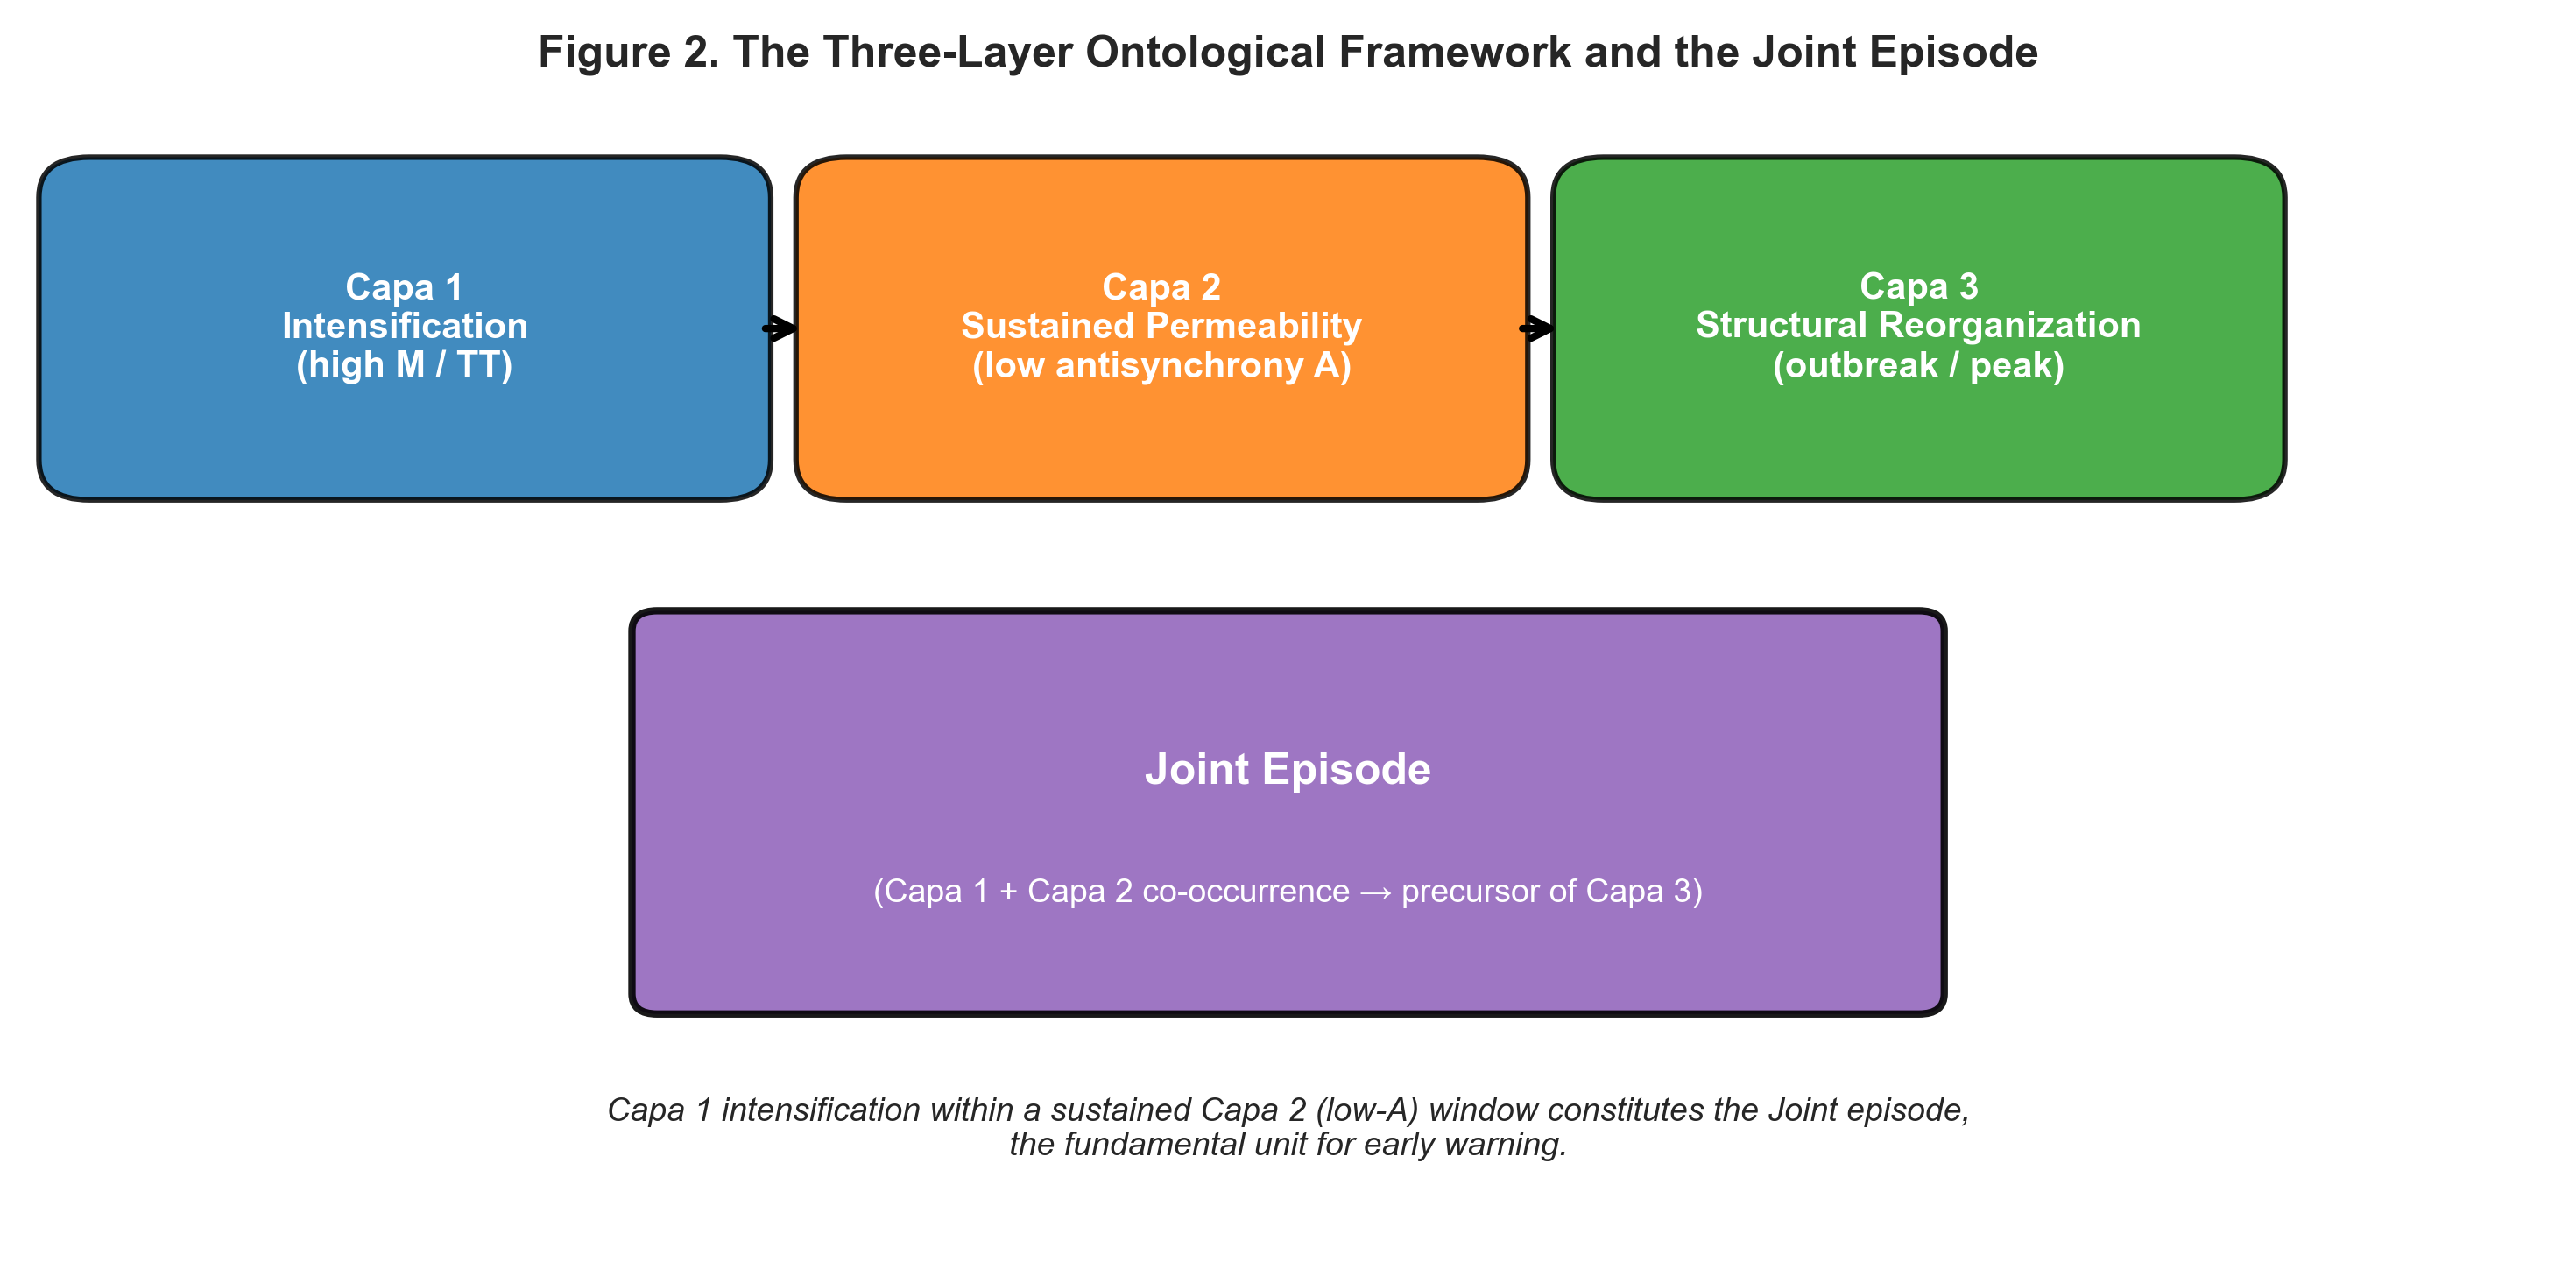
\includegraphics[width=0.92\textwidth]{figures/fig2_three_layer_framework.png}
\caption{Figure 1. The Three-Layer Ontological Framework and the Joint Episode. Capa 1 intensification within sustained Capa 2 permeability defines the Joint episode—the primary early-warning unit. Their co-occurrence raises the probability of Capa 3 reorganization.}
\label{fig:framework}
\end{figure}

\section{Data and RECD Features}

We employ publicly available DengAI datasets for San Juan and Iquitos. Recurrence-based features (M, trapping time, laminarity, and derived antisynchrony) were extracted using standard RQA procedures applied to incidence series.

A relaxed detector identifies Joint episodes as periods of low antisynchrony (A $<$ 0.05) lasting at least eight consecutive weeks that contain at least one high-M or high-trapping-time observation. From each episode we extract duration, mean\_M, Joint Score, and Capa 1 consistency.

In the examined windows, only 11 Joint episodes were identified for San Juan (empirical success rate to Capa 3 $\approx$ 0.73) and three for Iquitos. This scarcity, especially pronounced in Iquitos, precludes robust calibration or regime comparison from real data alone and motivates the synthetic component of the analysis.

\section{Methods: Pipeline Development (Phases 1--7)}

The methodological development proceeded through seven phases whose central decisions were guided by the three-layer ontology.

Phases 1--3 established the operational definition of the Joint episode. Systematic sensitivity analyses demonstrated that a relaxed criterion—sustained low antisynchrony containing high-M excursions—outperformed strict per-timestep coincidence in both lead time and coverage of Capa 3 events.

Phases 4--6 addressed prediction and operational utility. A random-forest model was trained on episode-derived and rolling recurrence features using temporal walk-forward validation. Operational utility was defined as a composite of lead-time benefit, false-positive cost, Capa 3 coverage, and alert burden. Episode-level aggregation (one alert per Joint episode) consistently outperformed per-step alerting. Phase 6 incorporated persistence and cooldown rules appropriate for public-health response.

Phase 7 introduced the Confidence Score:

\begin{sloppypar}
\[
\text{Confidence Score} = w_1 \cdot P(\text{C3} \mid \text{features}) + w_2 \cdot \text{Joint Score (norm.)} + w_3 \cdot \text{Duration (norm.)} + w_4 \cdot \text{Capa 1 consistency}
\]
\end{sloppypar}

Default weights (0.40, 0.25, 0.15, 0.20) were combined with fixed categorization thresholds (Alto $\geq$ 0.72, Medio $\geq$ 0.45). The score and its categories were designed to be directly interpretable as graded evidence that a Capa 1 + Capa 2 configuration is maturing toward reorganization.

\section{Synthetic Validation and Confidence Score Calibration (Phase 8)}

Real data contain too few observed Joint episodes to permit stable weight selection or probability calibration, and lack the controlled variation needed to test whether differences between sites reflect mere prevalence or qualitatively distinct layer dynamics. Synthetic generation was therefore required on ontological grounds: only by systematically varying the parameters that define Capa 1 intensity and Capa 2 persistence can we isolate the contribution of each layer and determine whether site differences are differences of degree or of kind.

The generator samples duration, mean\_M, and Capa 1 consistency from regime-specific distributions, computes the Joint Score, and derives a latent transition probability to Capa 3 via a logistic function of normalized intensity. Observational noise is injected to mimic features a real system would record. Three regimes were produced:

\begin{itemize}
    \item San Juan-like: long duration, high mean\_M, higher base transition rate.
    \item Iquitos-like: short duration, lower mean\_M, low base transition rate reflecting rare sustained Capa 2.
    \item Noisy balanced: intermediate statistics with elevated noise.
\end{itemize}

A grid of six weight vectors was evaluated on 2,200 synthetic episodes using Brier score, ROC-AUC, and F1 for the “Alto” category. This design enables direct, ontologically grounded comparisons of calibration and categorical behavior that the sparse real episodes cannot support.

\section{Results}

\subsection{Characteristics of Synthetic Regimes}

The generator reproduced the expected ontological contrast. San Juan-like episodes exhibited mean duration of 85 weeks (SD 51), mean Joint Score of 80.6, and mean\_M of 0.945, with a Capa 3 transition rate of 49.4\%. Iquitos-like episodes were markedly shorter (mean duration 25 weeks, SD 15), weaker (mean Joint Score 8.1, mean\_M 0.575), and less likely to transition (33.3\%). These statistics align with the sparse empirical record.

\begin{figure}[htbp]
\centering
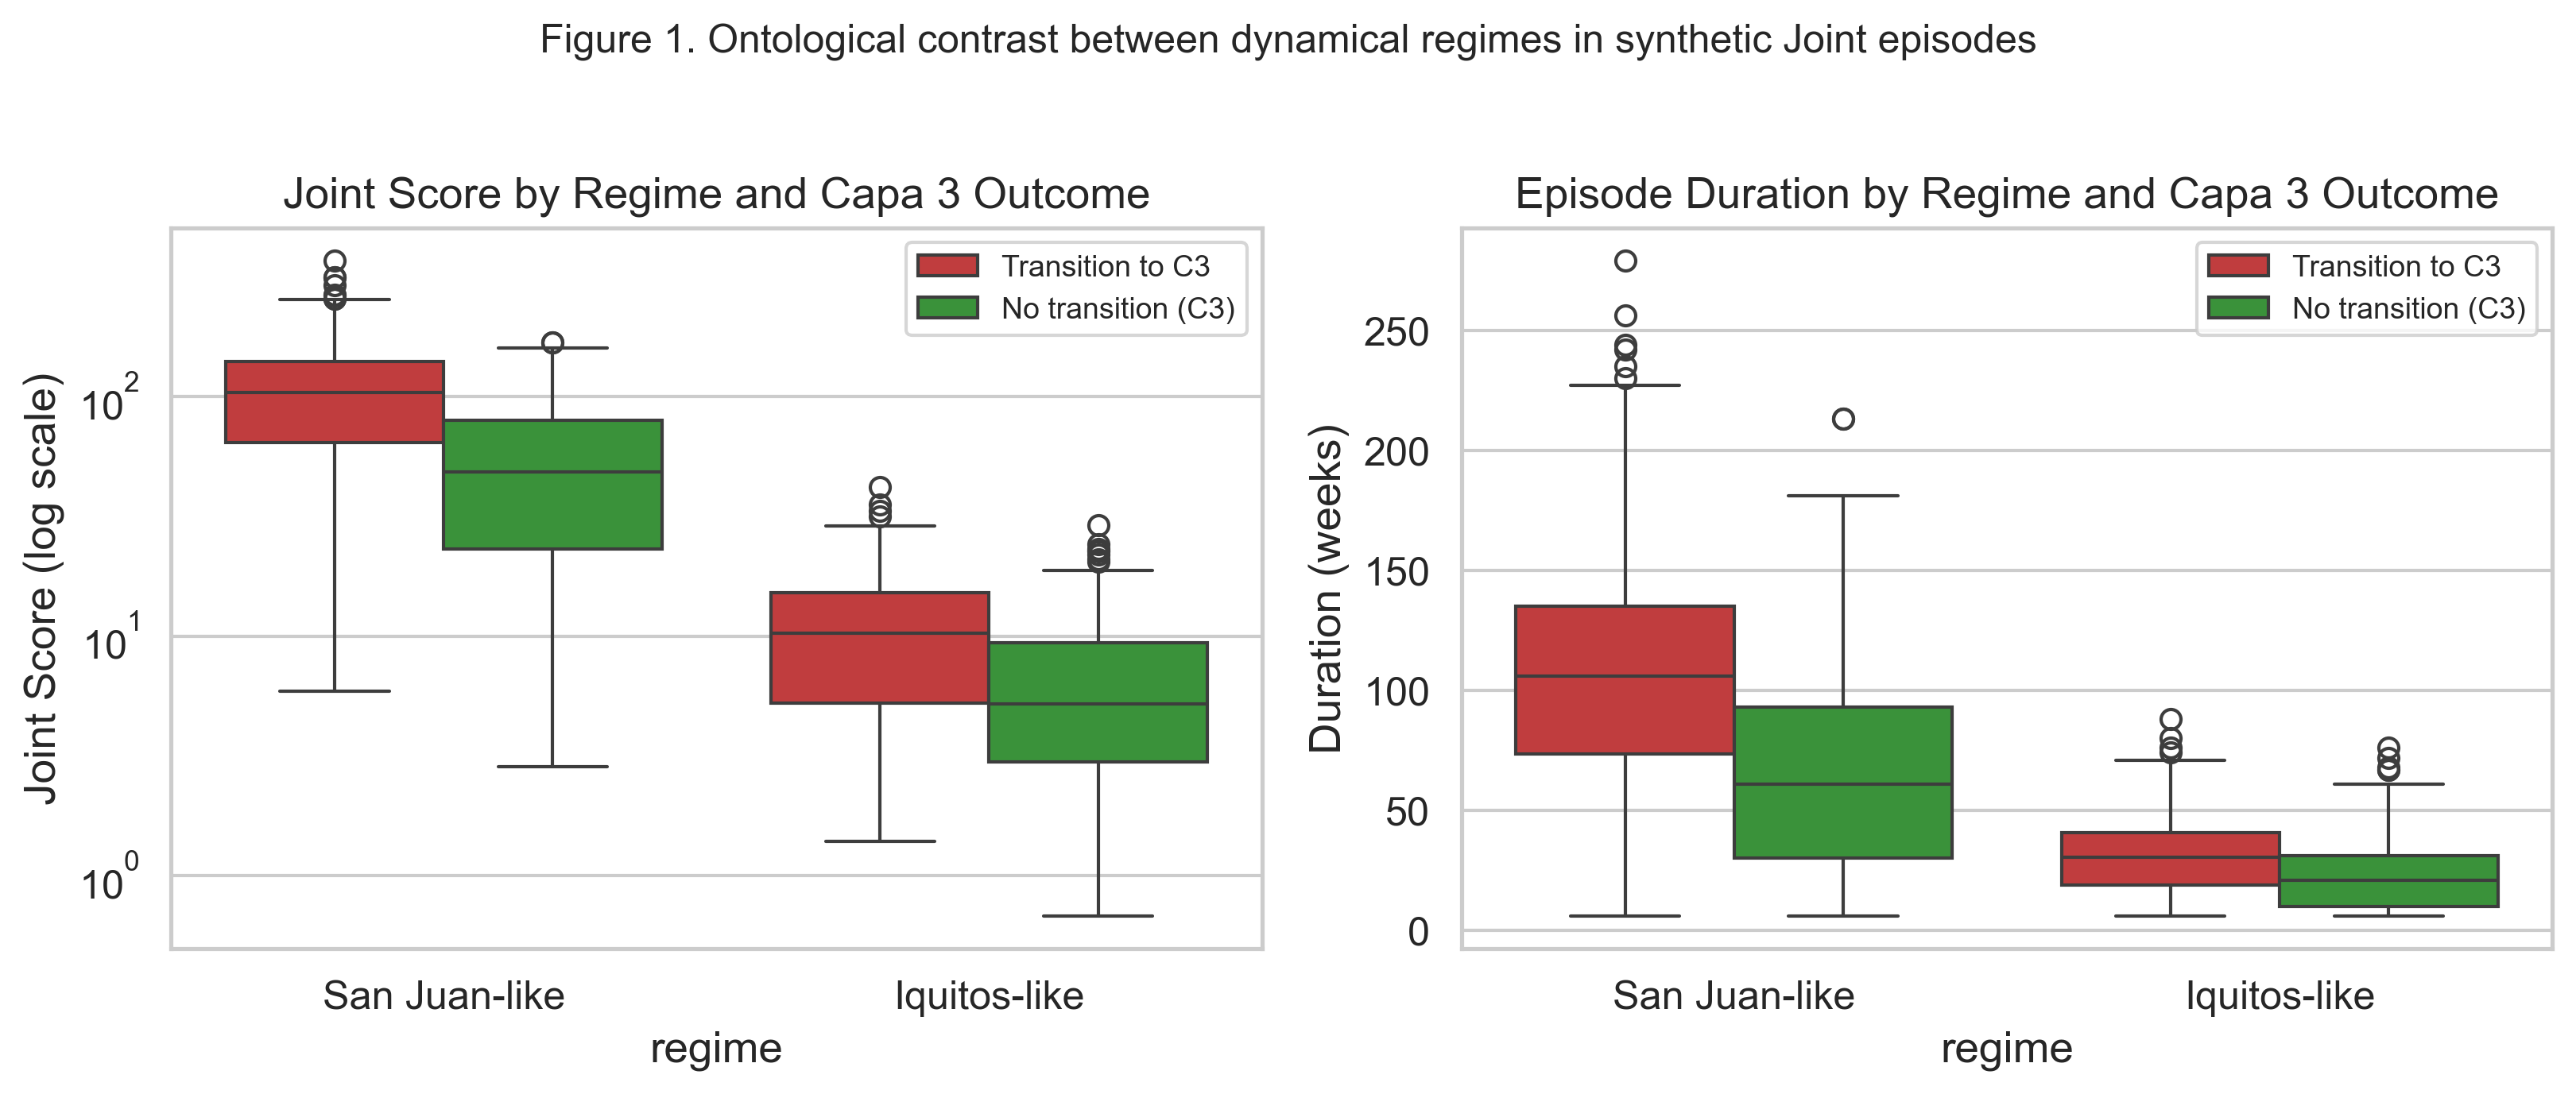
\includegraphics[width=\textwidth]{figures/fig1_regime_contrast.png}
\caption{Figure 2. Ontological contrast between dynamical regimes. Boxplots of Joint Score (log scale) and duration, stratified by regime and Capa 3 outcome. San Juan-like episodes are longer and stronger with clear outcome separation; Iquitos-like episodes are short and weak, indicating a distinct regime.}
\label{fig:regimes}
\end{figure}

\subsection{Confidence Score Performance Across Regimes}

Across all synthetic episodes, Brier scores ranged from 0.211 to 0.241 and AUC values from 0.64 to 0.75. Performance on the operationally critical “Alto” category diverged sharply by regime.

In the San Juan-like regime, weight vectors assigning substantial weight to Joint Score and duration achieved the highest Alto F1 (up to 0.55). Configurations emphasizing duration or the product of duration and intensity were particularly effective.

In the Iquitos-like regime, no weighting produced any “Alto” classifications (Alto F1 = 0). Mean confidence across episodes remained low (0.214--0.258). Even the most permissive weight vectors generated at most a small number of “Medio” episodes. The noisy balanced regime produced intermediate results consistent with the ranking observed under high-prevalence conditions.

\begin{figure}[htbp]
\centering
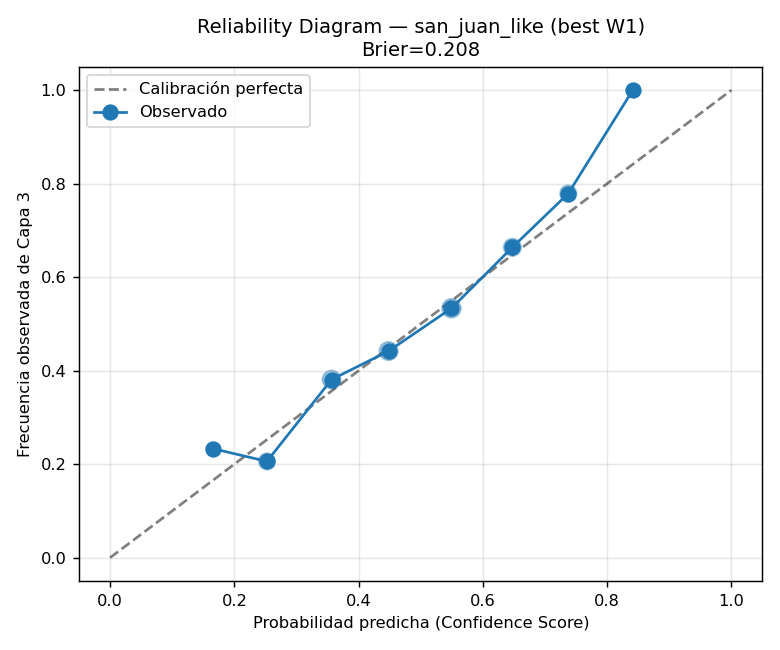
\includegraphics[width=0.48\textwidth]{figures/reliability_san_juan_like.png}
\hfill
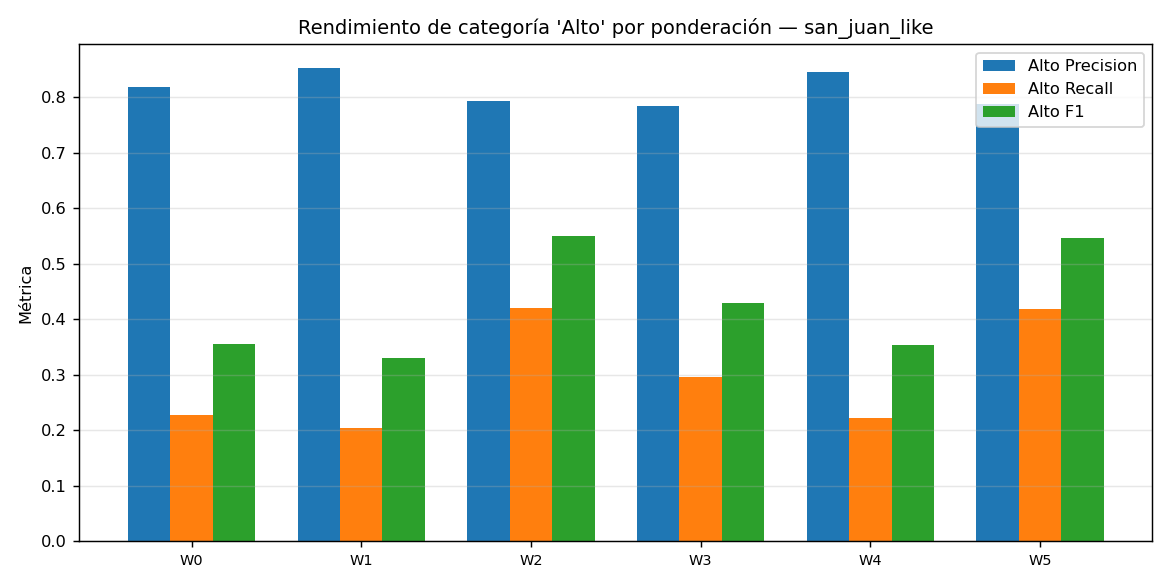
\includegraphics[width=0.48\textwidth]{figures/category_perf_san_juan_like.png}
\caption{Figure 3 (left). Calibration diagram (San Juan-like regime). Observed Capa 3 frequency vs. binned Confidence Score. Figure 4 (right). “Alto” category performance. Iquitos-like regime yields almost no “Alto” classifications.}
\label{fig:calib}
\end{figure}

Reliability diagrams indicated that the synthetic ground-truth transition probabilities were recoverable with modest bias, supporting future isotonic recalibration once larger real samples become available.

\subsection{Real-Data Context and Operational Implications}

The 11 Joint episodes recovered for San Juan and three for Iquitos yielded apparently high success rates but are too few for stable parameterization. Episode-level alerts with categorical output reduce notification volume by more than an order of magnitude relative to per-week models while preserving coverage of Capa 3 events in high-prevalence conditions. The “Alto” category concentrates those episodes most likely to warrant prioritized response.

\section{Discussion}

The synthetic results demonstrate that the three-layer framework does more than organize recurrence features; it exposes heterogeneity in how Capa 1 and Capa 2 interact across settings. The central finding is that the near-absence of high-confidence Joint episodes under Iquitos-like parameters is not merely an artifact of small sample size. It indicates that sustained Capa 2 states—periods of low antisynchrony long enough to contain Capa 1 intensification—are intrinsically rarer or shorter in that environment.

This difference carries ontological weight. It suggests that the conditions required for the permeability layer (Capa 2) to persist long enough for reorganization (Capa 3) are not uniformly distributed across locations. Contributing factors may include vector ecology, urban form, climatic seasonality, or mobility patterns that constrain the spatial or temporal extent of low-antisynchrony windows. Treating Iquitos simply as “data-poor San Juan” would therefore misrepresent the underlying layer dynamics and risk inappropriate threshold or feature choices.

The Confidence Score’s sensitivity to duration and Joint Score under high-prevalence conditions further shows the value of anchoring weights in the ontology. These components directly quantify the persistence and integrated force of the Capa 1 + Capa 2 configuration. In this way the framework converts a methodological necessity—synthetic data—into an empirical discovery of regime heterogeneity with immediate consequences for site-specific operational design.

Limitations remain. The generator relies on proxy probabilities and does not yet incorporate intervention covariates or serotype dynamics. Real external validation with extended Puerto Rico data and operational ground truth remains essential.

\section{Conclusions and Future Work}

We have developed and internally validated an ontologically grounded early-warning pipeline for dengue in which the Joint episode functions as the primary unit of analysis. Controlled synthetic generation proved essential for calibrating the Confidence Score and for demonstrating that differences between San Juan and Iquitos reflect distinct dynamical regimes rather than sampling limitations alone.

\textbf{Recommendations for Phase 9 and deployment:}
\begin{enumerate}
    \item Begin with duration- or Joint-Score-weighted configurations for San Juan-like settings; recalibrate with extended real data.
    \item For Iquitos-like contexts, consider modestly lower “Alto” thresholds or auxiliary indicators of Capa 2 persistence while actively acquiring additional data.
    \item Prioritize extended historical series and operational response records for Puerto Rico municipalities.
    \item Implement isotonic recalibration once 50--100 real Joint episodes are available.
    \item Design a prospective pilot in San Juan, where episode density supports stable evaluation.
\end{enumerate}

The framework is generalizable to other systems in which recurrence signatures of intensification and permeability precede observable reorganization.

\section*{Data and Code Availability}
\addcontentsline{toc}{section}{Data and Code Availability}

All code for Phases 1--8, the synthetic episode generator, weight-grid evaluation routines, and supporting scripts are available in the project repository:

\textbf{\url{https://github.com/johelpadilla/ontologia-presente}} (see subdirectory \texttt{preprints/\\recd\_dengue\_joint\_episodes\_2026}).

Synthetic episode datasets (2,200 episodes), calibration tables, reliability plots, the external validation protocol, and planning documents are included in this subfolder. Real incidence data are from the public DengAI competition.

\section*{References}
\addcontentsline{toc}{section}{References}
\begin{thebibliography}{99}

\bibitem{dengai}
DengAI: Predicting Disease Spread. DrivenData competition dataset, 2015--2016.

\bibitem{marwan2007}
Marwan, N., Romano, M. C., Thiel, M., \& Kurths, J. (2007). Recurrence plots for the analysis of complex systems. \textit{Physics Reports}, 438(5-6), 237--329.

\bibitem{scheffer2009}
Scheffer, M., et al. (2009). Early-warning signals for critical transitions. \textit{Nature}, 461(7260), 53--59.

\bibitem{tau2026}
Technical reports of the Tau Sistémico / RECD project – Joint Condition Characterization (Phases 1--8), 2025--2026.

\end{thebibliography}

\vspace{0.8em}
\hrule
\vspace{0.5em}
\noindent\textit{Supplementary Material:} Code, synthetic datasets, figures, the external validation protocol, and detailed planning documents are provided in the repository subfolder \texttt{preprints/recd\_dengue\_joint\_episodes\_2026} at \url{https://github.com/johelpadilla/ontologia-presente}.

\vspace{0.6em}
\noindent\textit{Preprint deposited on Zenodo – June 2026. Version 1.2.}  
\noindent\textit{Author: Dr. Johel Padilla Villaunueva.}

\end{document}